\section{Gestione amministrativa della revisione}
\sectionmark{Gestione amministrativa \dots}
% APPROFONDIRE da Sommerville capitolo 24, paragrafo 24.4.2 Software compoent analisys

	\subsection{Comunicazione delle anomalie}
	\label{DefinizioneAnomalie}

	Il processo di \glossario{Software Quality Managment} è finalizzato alla ricerca dei difetti. L'identificazione delle anomalie ne permette la correzione e informa il \emph{Responsabile} di progetto sullo stato del prodotto. Distinguere e catalogare le anomalie è utile per discutere durante revisioni e riunioni su che correzioni attuare e con quale priorità. Di seguito vengono elencate le definizioni di anomalie (IEEE 610.12-90) adottate dal gruppo:
	\begin{itemize}
		\item \textbf{Error}: differenza riscontrata tra il risultato di una computazione e il valore teorico atteso (e.g. uscita dal range di accettazione degli indici di misurazione);
		\item \textbf{Fault}: un passo, un processo o un dato definito in modo erroneo (e.g. violazioni di norme tipografiche da parte di un documento). Corrisponde a quanto viene definito come \glossario{bug};
		\item \textbf{Failure}: il risultato di un \emph{fault} (e.g. incongruenza del prodotto con funzionalità indicate nell'analisi dei requisiti, incongruenza del codice con il design del prodotto);
		\item \textbf{Mistake}: azione umana che produce un risultato errato (e.g. anomalie nel repository).
	\end{itemize}
	La catalogazione delle anomalie permette l'impostazione di metriche in grado di valutarne l'andamento e in alcuni casi di predirlo. In particolare è stata scelta la metrica che conteggia il numero di \emph{\glossario{bug} per lines of code}. Il \glossario{SCR} (software change request) utilizzato dal gruppo viene individuato nelle \NormeDiProgetto.


	\subsection{Controlli per la qualità di processo}
	% potrebbe evolvere in un Appendice escluisvamente dedicata alla qualità

	Le procedure di controllo per la qualità di processo sono finalizzate a migliorare la qualità del prodotto e/o diminuire i costi e tempi di sviluppo. Esistono due approcci principali:
	\begin{itemize}
		\item \textbf{A maturità di processo}: riflette le buone pratiche di management e tecniche di sviluppo. L'obiettivo primario è la qualità del prodotto e la prevedibilità dei processi;
		\item \textbf{Agile}: sviluppo iterativo senza l'overhead della documentazione e di tutti gli aspetti predeterminabili. Ha come caratteristica la responsività ai cambiamenti dei requisti cliente e uno sviluppo rapido.
	\end{itemize}

	Verrà utilizzato il primo approccio, in quanto più adatto ad un team inesperto. Con una visione proattiva si cerca di avere maggior controllo e previsione sulle attività da svolgere. Questa viene anche indicata come \glossario{best practice} per gruppi poco esperti.\\
	Il processo con maggiore influenza sulla qualità del sistema non è quello di sviluppo ma quello di progettazione. È qui che le capacità e le esperienze dei singoli danno un contributo decisivo.\\
	Il miglioramento dei processi è un processo ciclico composto da tre sotto-processi:
	
	\begin{figure}[h]
	\centering 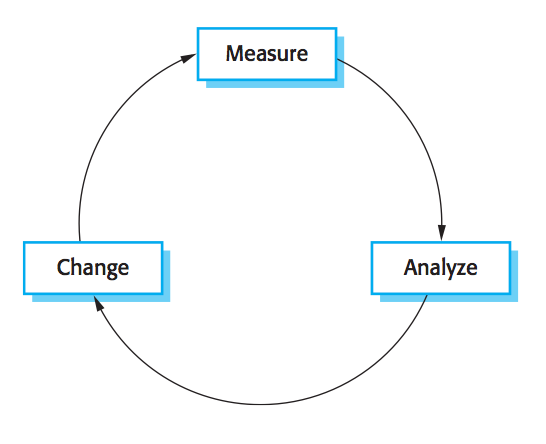
\includegraphics[width=0.8\textwidth]{ProcessImprovementCycle.png}
	\caption{Il ciclo di miglioramento dei processi}
	\end{figure}

	\begin{itemize}
		\item Misurazione del processo: misura gli attributi del progetto, punta ad allineare gli obiettivi con le misurazioni effettuate. Questo forma una \glossario{baseline} che aiuta a capire se i miglioramenti hanno avuto effetto;
		\item Analisi del processo: vengono identificate le problematiche ed i colli di bottiglia dei processi;
		\item Modifiche del processo: i cambiamenti vengono proposti in risposta alle problematiche riscontrate.
	\end{itemize}
	
	Il gruppo procederà nel seguente modo: 
	\begin{itemize}
		\item Nella sezione \emph{Dettaglio delle verifiche tramite analisi} (\ref{DettaglioVerificheAnalisi}) verranno inserite le misurazioni rilevate sulle le metriche descritte in \emph{Misure e Metriche} (\ref{MisureMetriche});
		\item L'analisi viene effettuata i giorni precedenti alle consegne previste dal committente; il \emph{Riassunto delle attività di verifica} (\ref{RiassuntoAttivitaVerifica}) contiene l'analisi del processo, le relative considerazioni  comprendenti le problematiche riscontrate;
		\item Le modifiche al processo vengono attuate all'inizio del processo incrementale successivo. Queste attività sono programmate nel \PianoDiProgetto.
	\end{itemize}
	
	
	
	
	
